The \textbf{Map Component} is one of the most critical components in SeatGen, responsible for rendering and managing the stadium seating map. It integrates with \textbf{Leaflet.js} to provide interactive seat visualization, selection, and manipulation.

\textbf{Key Responsibilities:}
\begin{itemize}
    \item Initializes and manages the \textbf{Leaflet map instance}.
    \item Loads seat and standing area data dynamically from the backend.
    \item Renders seats and standing areas as \textbf{interactive markers and polygons}.
    \item Handles user interactions such as \textbf{clicking, selecting, and dragging seats}.
    \item Implements \textbf{state synchronization} with the global context (\textbf{Map Context}).
    \item Provides support for \textbf{tool-based seat editing} (e.g., adding, deleting, moving).
\end{itemize}

\textbf{Component Structure:}
\begin{itemize}
    \item \textbf{State Management:} Uses \texttt{useState}, \texttt{useEffect}, and \texttt{useContext} to manage map data.
    \item \textbf{Leaflet Integration:} Utilizes \texttt{MapContainer} from \texttt{react-leaflet} for seamless map rendering.
    \item \textbf{Performance Enhancements:} Implements \texttt{useCallback} and \texttt{useRef} to optimize re-renders.
\end{itemize}

\subsubsection{Map Initialization and Leaflet Integration}

The \textbf{Map Component} initializes the Leaflet map using the react-leaflet \texttt{MapContainer} component.

\begin{lstlisting}[language=TypeScript, caption=Initializing Leaflet Map in React, label=lst:react-leaflet]
const MapComponent: FC<MapProps> = ({ editable: initialEditable }) => {
    const context = useMapContext(); // Access global state (Map Context)
    const { bucketName, mapName } = useParams(); // Retrieve map identifiers from URL params

    const [editable, setEditable] = useState(initialEditable ?? true);
    const mapRef = useRef<L.Map>(null);

    return (
        <MapContainer
            crs={L.CRS.Simple} // Uses a flat, pixel-based coordinate system
            className="leaflet-container h-full w-full"
            ref={mapRef}
            center={[context.mapInfo.tileSize / (-2), context.mapInfo.tileSize / (2)]}
            zoom={context.mapInfo.defaultZoom}
            maxZoom={context.mapInfo.maxZoom}
            minZoom={context.mapInfo.minZoom}
            scrollWheelZoom={true}
            zoomControl={false}
            doubleClickZoom={false}
            preferCanvas={true}
            dragging={true}
            tap={false}
            renderer={L.canvas()} // Use Canvas for better performance
        >
            <TileLayer tms={true} url={`${context.mapInfo.mapDto.baseUrl}/{z}/{x}/{y}.png`} />
        </MapContainer>
    );
};
\end{lstlisting}

\textbf{Custom CRS (Coordinate Reference System):}
\begin{itemize}
    \item Uses \textbf{L.CRS.Simple}, a \textbf{2D pixel-based coordinate system}.
    \item Unlike traditional geographic maps, SeatGen does not need a curved map.
    \item All coordinates can be converted to a Cartesian X/Y grid.
\end{itemize}

\textbf{Custom Rendering Engine:}
\begin{itemize}
    \item Uses \textbf{L.canvas()} instead of SVG for performance.
    \item Enables handling of thousands of seat markers.
    \item Reduces DOM load by rendering elements in a drawing surface.
\end{itemize}

\textbf{Dynamically Loading Map Tiles:}
\begin{itemize}
    \item The tile URL is dynamically constructed based on \texttt{context.mapInfo}.
    \item Tiles are loaded asynchronously to improve map load times.
\end{itemize}


\subsubsection{Fetching Seat and Standing Area Data}
\setauthor{Michael Ruep}

The Map Component fetches seat and standing area data from the backend when the component mounts. This is done using the api client in the useEffect hook.

\begin{lstlisting}[language=TypeScript, caption=Fetching Seat and Category Data, label=lst:fetch-seats]
useEffect(() => {
    if (bucketName && mapName) {
        // Fetch basic stadium map information
        seatgenApiClient.api.info(bucketName, mapName)
            .then(response => context.setMapInfo(response.data))
            .catch(error => console.error('Error fetching map info:', error));

        // Fetch seat categories before retrieving individual seats
        seatgenApiClient.api.getAllCategories().then((r) => {
            if (r.ok) {
                context.setCategories(r.data);
                seatgenApiClient.api.getSeatsByMap(bucketName, mapName).then(response => {
                    if (r.ok) {
                        context.setSeats(response.data.map((s) => ({
                            id: s.seatId!,
                            position: { lat: s.xcoord!, lng: s.ycoord! },
                            category: r.data.find(it => it.id === s.categoryId) ?? null
                        })));
                    }
                });
            }
        });

        // Fetch standing areas
        seatgenApiClient.api.getSectorByMap(bucketName, mapName).then((r) => {
            if (r.ok) {
                context.setStandingAreas(r.data.map((data) => ({
                    id: data.id!,
                    name: data.name!,
                    capacity: data.capacity,
                    coordinates: data.coordinates?.map((c) => new L.LatLng(c.x!, c.y!)) ?? [],
                    selected: false
                })));
            }
        });

    } else {
        console.error("BucketName or MapName not set");
    }
}, [bucketName, mapName]);
\end{lstlisting}

\textbf{Breakdown of Logic:}
\begin{itemize}
    \item Fetches stadium metadata (mapInfo) and sets it globally.
    \item Retrieves seat categories.
    \item Retrieves seat positions from the backend and maps them into React state.
    \item Ensures data consistency by linking seats to their corresponding categories.
\end{itemize}

\textbf{Example of Mapped Seat Object:}
\begin{lstlisting}[language=TypeScript, caption=Seat Object in State, label=lst:seat-object]
{
    id: 1234,
    position: { lat: 48.3069, lng: 14.2858 }, // Example coordinates
    category: { id: 2, name: "VIP", color: "#FFD700" } // Associated category
}
\end{lstlisting}

\subsubsection{Fetching Standing Area / Sector Data}
In addition to seats, the component also retrieves standing areas, which are handled separately.

\begin{lstlisting}[language=TypeScript, caption=Fetching Standing Areas, label=lst:fetch-standingareas]
seatgenApiClient.api.getSectorByMap(bucketName, mapName).then((r) => {
    if (r.ok) {
        context.setStandingAreas(r.data.map((data) => ({
            id: data.id!,
            name: data.name!,
            capacity: data.capacity,
            coordinates: data.coordinates?.map((c) => new L.LatLng(c.x!, c.y!)) ?? [],
            selected: false
        })));
    }
});
\end{lstlisting}

\textbf{Explanation:}
\begin{itemize}
    \item The API returns a list of sector polygons.
    \item Each area consists of a unique ID, name, capacity, and a list of coordinates.
    \item Coordinates are transformed into Leaflet’s LatLng format to be rendered as a polygon.
\end{itemize}

\textbf{Example of a Standing Area Object in State:}
\begin{lstlisting}[language=TypeScript, caption=Standing Area Object in State, label=lst:standingarea-object]
{
    id: 69420,
    name: "Sektor 69",
    capacity: 187,
    coordinates: [
        { lat: 48.3069, lng: 14.2858 },
        { lat: 48.3075, lng: 14.2862 },
        { lat: 48.3080, lng: 14.2856 }
    ],
    selected: false
}
\end{lstlisting}

\subsubsection{State Management and Performance}
\begin{itemize}
    \item \texttt{useEffect} Dependency Array:
    \begin{itemize}
        \item Ensures the API calls only run when \texttt{bucketName} or \texttt{mapName} change.
        \item Prevents unnecessary re-fetching on every render.
    \end{itemize}
    
    \item Efficient State Updates:
    \begin{itemize}
        \item Avoids unnecessary re-renders by batching state updates for seats and standing areas.
        \item No prop-drilling by storing fetched data needed globally in the \texttt{Map Context}.
    \end{itemize}

    \item Error Handling:
    \begin{itemize}
        \item If any API call fails, an error is logged, and the operation is skipped.
        \item Ensures that failures in one request do not crash the entire component.
    \end{itemize}
\end{itemize}

\subsubsection{Rendering Seats and Handling Selection}
\setauthor{Michael Ruep}

Each seat in the stadium is rendered as a Leaflet marker, allowing users to interact with them dynamically. The selection mechanism is designed to provide an intuitive experience while supporting multi-selection for bulk operations.

\textbf{Rendering Seat Markers:}
\begin{lstlisting}[language=TypeScript, caption=Rendering and Selecting Seats, label=lst:seat-rendering]
const handleSeatClick = useCallback((id: number, event: L.LeafletMouseEvent) => {
    const isCtrlPressed = event.originalEvent?.ctrlKey;

    context.setSeats(prevSeats => prevSeats.map(seat => {
        if (seat.id === id) {
            const selected = isCtrlPressed ? !seat.selected : true;
            return { ...seat, selected };
        }
        return isCtrlPressed ? seat : { ...seat, selected: false };
    }));

    setOpenSideBar(true);
}, [context]);
\end{lstlisting}

\textbf{How This Works:}
\begin{itemize}
    \item Clicking a seat toggles its selected state.
    \item Holding \textbf{Ctrl} allows multi-selection, useful for bulk actions.
    \item Clicking a seat opens the \textbf{DetailEditor sidebar} for further modifications.
\end{itemize}


\subsubsection{Implementing Live Seat Dragging and Moving}
\setauthor{Michael Ruep}

In SeatGen, users can drag and reposition multiple selected seats dynamically. The challenge was ensuring that \textbf{all} selected seats move smoothly and live directly following the cursor while keeping their relative distances intact. To achieve this, a real-time position tracking mechanism was implemented using Leaflet events and React state updates.

\subsubsection{Tracking Initial Positions}
Before moving seats, their initial positions are stored so that relative offsets can be preserved:

\begin{lstlisting}[language=TypeScript, caption=Storing Initial Positions Before Dragging, label=lst:seat-initial-pos]
const initialPositionsRef = useRef<{ [key: number]: L.Point }>({});

const storeInitialPositions = useCallback(() => {
    const map = mapRef.current;
    if (!map) return;

    initialPositionsRef.current = {};
    selectedSeats.forEach(seat => {
        initialPositionsRef.current[seat.id] = map.latLngToLayerPoint(seat.position);
    });

    // Register move action for undo functionality
    context.doAction(new MoveAction(selectedSeats, context.setSeats));
}, [selectedSeats, context]);
\end{lstlisting}

\textbf{How This Works:}
\begin{itemize}
    \item A reference (\texttt{initialPositionsRef}) is created to store the pixel positions of selected seats by converting the Latitude and Longitude into Layer Points which are x and y Cartesian System points.
    \item These positions are saved when the user starts dragging a seat.
    \item The relative distance between seats is maintained, preventing unwanted misalignment.
\end{itemize}

\subsubsection{Updating Seats in Real-Time During Dragging}
While the user drags a seat, the drag distance is calculated and applied to all selected seats:

\begin{lstlisting}[language=TypeScript, caption=Updating Seat Positions During Dragging, label=lst:seat-live-dragging]
const updateSelectedSeatsPosition = useCallback((draggedSeatId: number, newLatLngPosition: { lat: number; lng: number }) => {
    const map = mapRef.current;
    const primarySeat = context.seats.find(s => s.id === draggedSeatId);

    if (!map || !primarySeat || !primarySeat.selected) return;

    const newPosition = map.latLngToLayerPoint(newLatLngPosition);
    const oldPosition = initialPositionsRef.current[draggedSeatId];

    const deltaX = newPosition.x - oldPosition.x;
    const deltaY = newPosition.y - oldPosition.y;

    context.setSeats(prevSeats =>
        prevSeats.map(seat => {
            if (seat.selected) {
                const initialPosition = initialPositionsRef.current[seat.id];
                const newPosX = initialPosition.x + deltaX;
                const newPosY = initialPosition.y + deltaY;
                const newLatLngPos = map.layerPointToLatLng(new L.Point(newPosX, newPosY));
                return { ...seat, position: newLatLngPos };
            }
            return seat;
        })
    );

    // Update MoveAction for undo tracking
    const currentAction = context.getCurrentAction();
    if (currentAction instanceof MoveAction) {
        currentAction.setNewSeats(selectedSeats);
    }
}, [context.seats, context]);
\end{lstlisting}

\textbf{Breakdown of Logic:}
\begin{itemize}
    \item The drag delta (change in X/Y position) between the starting position and the new cursor position is calculated.
    \item The same delta is applied to all selected seats, ensuring they move together.
    \item Positions are converted between LatLng (geo-coordinates) and pixel points, so dragging works consistently at different zoom levels.
    \item Changes using \texttt{MoveAction} are tracked, allowing the operation to be undone if needed.
\end{itemize}

\subsubsection{Optimizations and Challenges}
\textbf{Major Challenges Encountered:}
\begin{itemize}
    \item Preventing position drift when switching between zoom levels.
    \item Ensuring smooth movement with large seat selections.
    \item Avoiding excessive re-renders that slow down performance.
\end{itemize}

\textbf{Performance Optimizations:}
\begin{itemize}
    \item Used \texttt{useRef} to store initial positions instead of state (prevents extra re-renders).
    \item Applied batch updates for all selected seats instead of updating them individually.
    \item Optimized Leaflet latLng-to-pixel conversion to enable natural seat dragging (direct manipulation \cite{Hutchins01121985}).
\end{itemize}

\subsubsection{Conclusion}
The live dragging implementation allows users to dynamically reposition multiple seats while keeping their relative distances intact. By leveraging Leaflet’s coordinate system and real-time state updates, a fluid and high-performance dragging experience was achieved, with full undo and redo functionality.

\subsubsection{Managing Standing Areas and Sectors}
\setauthor{Michael Ruep}

SeatGen allows the definition of standing areas / sectors, which differ from regular seats by not being assigned individual markers but instead represented as polygonal sectors. Each standing area has a defined capacity, ensuring ticketing restrictions.

\textbf{Standing Area Features:}
\begin{itemize}
    \item \textbf{Custom Polygons:} Users define standing areas by selecting points on the map.
    \item \textbf{Capacity Control:} Limits the number of tickets available per standing area.
    \item \textbf{Category Assignment:} Standing areas can be assigned different categories.
    \item \textbf{Real-time Editing:} Areas can be renamed, and deleted dynamically.
\end{itemize}

\textbf{Standing Area Selection:}
\begin{lstlisting}[language=TypeScript, caption=Handling Standing Area Selection, label=lst:select-standingareas]
const handlePolygonClick = useCallback((id: number, event: L.LeafletMouseEvent) => {
    const isCtrlPressed = event.originalEvent?.ctrlKey;

    // Deselect all seats when a polygon is clicked
    context.setSeats(prevSeats => prevSeats.map(seat => ({
        ...seat,
        selected: false
    })));

    const selectedStandingAreaIds: number[] = [];
    context.setStandingAreas(prevAreas => {
        return prevAreas.map(area => {
            if (area.id === id) {
                const selected = isCtrlPressed ? !area.selected : true;
                if (selected) selectedStandingAreaIds.push(area.id);
                return { ...area, selected };
            }
            if (!isCtrlPressed) {
                return { ...area, selected: false };
            }
            if (area.selected) selectedStandingAreaIds.push(area.id);
            return area;
        });
    });
    // Update the selected standing area IDs in context
    context.setSelectedStandingAreaIds(selectedStandingAreaIds);
    setOpenSideBar(true);
}, [context, setOpenSideBar]);
\end{lstlisting}

\textbf{Selection and Editing Process:}
\begin{itemize}
    \item Clicking a standing area toggles its selected state.
    \item In the Detail Editor panel, renaming, capacity adjustments, and category (including color coding) updates are possible.
\end{itemize}

\begin{figure}[H]
    \centering
    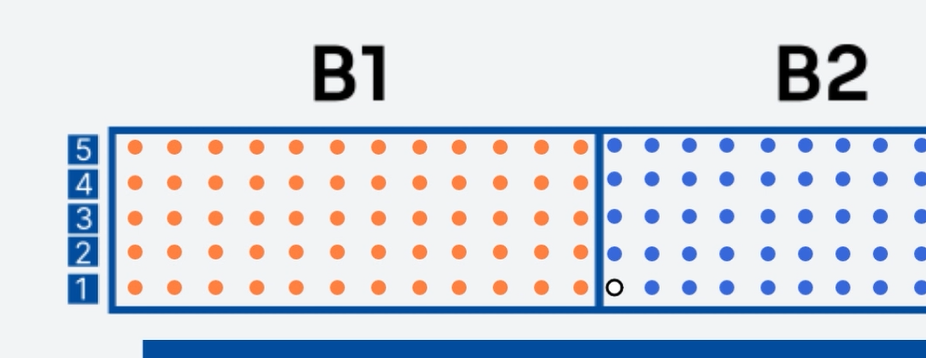
\includegraphics[width=0.7\textwidth]{pics/MapComponentCategoryAndSelectedSeat.png}
    \caption{Map, Seats with Category Color, and Selected Seat in Map Component}
    \label{fig:map-component-category}
\end{figure}

\subsubsection{Event Handling in Leaflet}
\setauthor{Michael Ruep}

SeatGen relies heavily on Leaflet event handling to manage user interactions dynamically. TODO Deselection
TODO Drag Events for Seat Movement + reference

\begin{lstlisting}[language=TypeScript, caption=Handling Seat Drag Events, label=lst:leaflet-seat-drag]
// Function definitions for handling drag events
const handleDragStart = (seatId: number) => {
    storeInitialPositions();
};

const handleDragEnd = (seatId: number, newPosition: L.LatLng) => {
    updateSelectedSeatsPosition(seatId, newPosition);
};

// Applying event listeners to each seat marker
const renderedSeats = useMemo(() => {
    return context.seats.map(seat => (
        <Seat 
            key={seat.id} 
            id={seat.id}
            position={seat.position} 
            updatePosition={updateSeatPosition}
            updateSelectedSeatsPosition={updateSelectedSeatsPosition}
            storeInitialPositions={storeInitialPositions} 
            tooltipText={seat.tooltipText}
            onClick={(event: LeafletMouseEvent) => handleSeatClick(seat.id, event)}
            onDragStart={() => handleDragStart(seat.id)}
            onDragEnd={(event) => handleDragEnd(seat.id, event.target.getLatLng())}
            draggable={editable}
            selected={seat.selected}
            category={seat.category}
        />
    ));
}, [context.seats, selectedSeats]);
\end{lstlisting}

\begin{itemize}
    \item The handleDragStart function is called when a user begins dragging a seat. It stores the initial positions of selected seats to ensure relative movement.
    \item The handleDragEnd function finalizes the new seat positions when dragging stops.
    \item Event listeners (onDragStart and onDragEnd) are added to each Seat component to trigger these functions dynamically.
    \item The useMemo hook optimizes rendering performance by ensuring seat markers are not unnecessarily re-created during re-renders.
\end{itemize}

\subsubsection{Saving and Syncing with the Backend}
\setauthor{Michael Ruep}
SeatGen implements an asynchronous saving mechanism that synchronizes data with the backend.

\textbf{Warning Users Before Leaving Without Saving:}

The \texttt{Leave Page Popup} component ensures that users are warned before navigating away from the application when they have unsaved changes. This prevents accidental data loss and provides an opportunity to save progress before exiting.

\begin{itemize}
    \item Detects unsaved changes via the \texttt{hasUnsavedChanges} prop.
    \item Attaches a \texttt{beforeunload} event listener to prevent accidental exits.
    \item Displays a native browser warning when users try to leave.
    \item Removes the event listener when no longer needed to optimize performance.
\end{itemize}

\begin{lstlisting}[language=TypeScript, caption=Auto-Saving on Unload, label=lst:auto-save-seats]
    interface FormPromptProps {
        hasUnsavedChanges: boolean;
    }
    
    export const LeavePagePopup: FC<FormPromptProps> = ({ hasUnsavedChanges }) => {
        useEffect(() => {
            const onBeforeUnload = (e: BeforeUnloadEvent) => {
                if (hasUnsavedChanges) {
                    e.preventDefault();
                    e.returnValue = "";
                }
            };
            window.addEventListener("beforeunload", onBeforeUnload);
            return () => {
                window.removeEventListener("beforeunload", onBeforeUnload);
            };
        }, [hasUnsavedChanges]);
    };
\end{lstlisting}


\textbf{How It Works:}
\begin{itemize}
    \item The \texttt{hasUnsavedChanges} prop determines whether to enable the warning.
    \item When unsaved changes are detected, a \texttt{beforeunload} event listener is added.
    \item If the user attempts to leave the page, the browser displays a warning.
    \item The event listener is removed when the component unmounts to prevent memory leaks.
\end{itemize}

\textbf{Batch Save:}
\begin{lstlisting}[language=TypeScript, caption=Batch Save Mechanism, label=lst:batch-save-seats]
const saveChanges = useCallback(() => {
    seatgenApiClient.api.saveSeats(bucketName, mapName, context.seats.map(seat => ({
        id: seat.id,
        x: seat.position.lat,
        y: seat.position.lng,
        categoryId: seat.category?.id
    })))
    .then(() => enqueueSnackbar("Changes saved successfully!", { variant: "success" }));
}, [context.seats]);
\end{lstlisting}

\textbf{Batch Save Mechanism:}
\begin{itemize}
    \item Instead of saving each individual seat change separately, SeatGen groups multiple seat updates into a single API request to reduce network overhead and improve efficiency.
    \item The \texttt{useCallback} hook ensures that changes get only saved when \texttt{context.seats} changes, preventing redundant function executions.
    \item \texttt{seatgenApiClient.api.saveSeats} sends the updated seat data to the backend, including the seat ID, coordinates, and category ID.
    \item Upon a successful save, a snackbar notification is displayed to confirm the operation.
    \item SeatGen maintains the action history so users can revert unintended changes before saving.
\end{itemize}

This saving mechanism ensures that the application remains responsive while keeping data integrity intact, even in scenarios where users forget to manually save their progress, they will be reminded.

\subsubsection{Summary}
The \textbf{Map Component} is the core of SeatGen’s interactive seating system. It efficiently manages:
\begin{itemize}
    \item Interactive Leaflet-based Map Rendering
    \item Seat and Standing Area Rendering
    \item Group Selection and Bulk Editing
    \item Drag-and-Drop Seat Repositioning
    \item Event Handling for User Interaction
    \item Synchronizing data with global state (\texttt{Map Context})
    \item Asynchronous Backend Synchronization
\end{itemize}

It ensures smooth operation even for large stadium layouts with thousands of seats.

